%%%%%%%%%%%%%%%%%%%%%%%%%%%%%%%%%%%%%%%
% Wenneker Resume/CV
% LaTeX Template
% Version 1.1 (19/6/2016)
%
% This template has been downloaded from:
% http://www.LaTeXTemplates.com
%
% Original author:
% Frits Wenneker (http://www.howtotex.com) with extensive modifications by 
% Vel (vel@LaTeXTemplates.com)
%
% License:
% CC BY-NC-SA 3.0 (http://creativecommons.org/licenses/by-nc-sa/3.0/
%
%%%%%%%%%%%%%%%%%%%%%%%%%%%%%%%%%%%%%%

%----------------------------------------------------------------------------------------
%	PACKAGES AND OTHER DOCUMENT CONFIGURATIONS
%----------------------------------------------------------------------------------------

\documentclass[a4paper,12pt]{memoir} % Font and paper size

%%%%%%%%%%%%%%%%%%%%%%%%%%%%%%%%%%%%%%%%%
% Wenneker Resume/CV
% Structure Specification File
% Version 1.1 (19/6/2016)
%
% This file has been downloaded from:
% http://www.LaTeXTemplates.com
%
% Original author:
% Frits Wenneker (http://www.howtotex.com) with extensive modifications by 
% Vel (vel@latextemplates.com)
%
% License:
% CC BY-NC-SA 3.0 (http://creativecommons.org/licenses/by-nc-sa/3.0/)
%
%%%%%%%%%%%%%%%%%%%%%%%%%%%%%%%%%%%%%%%%%

%----------------------------------------------------------------------------------------
%	PACKAGES AND OTHER DOCUMENT CONFIGURATIONS
%----------------------------------------------------------------------------------------

\usepackage{XCharter} % Use the Bitstream Charter font
\usepackage[utf8]{inputenc} % Required for inputting international characters
\usepackage[T1]{fontenc} % Output font encoding for international characters

\usepackage[top=1cm,left=1cm,right=1cm,bottom=1cm]{geometry} % Modify margins

\usepackage{graphicx} % Required for figures

\usepackage{flowfram} % Required for the multi-column layout

\usepackage{url} % URLs

\usepackage[usenames,dvipsnames]{xcolor} % Required for custom colours

\usepackage{tikz} % Required for the horizontal rule

\usepackage{enumitem} % Required for modifying lists
\setlist{noitemsep,nolistsep} % Remove spacing within and around lists

\setlength{\columnsep}{\baselineskip} % Set the spacing between columns

% Define the left frame (sidebar)
\newflowframe{0.2\textwidth}{\textheight}{0pt}{0pt}[left]
\newlength{\LeftMainSep}
\setlength{\LeftMainSep}{0.2\textwidth}
\addtolength{\LeftMainSep}{1\columnsep}
 
% Small static frame for the vertical line
\newstaticframe{1.5pt}{\textheight}{\LeftMainSep}{0pt}
 
% Content of the static frame with the vertical line
\begin{staticcontents}{1}
\hfill
\tikz{\draw[loosely dotted,color=RoyalBlue,line width=1.5pt,yshift=0](0,0) -- (0,\textheight);}
\hfill\mbox{}
\end{staticcontents}
 
% Define the right frame (main body)
\addtolength{\LeftMainSep}{1.5pt}
\addtolength{\LeftMainSep}{1\columnsep}
\newflowframe{0.7\textwidth}{\textheight}{\LeftMainSep}{0pt}[main01]

\pagestyle{empty} % Disable all page numbering

\setlength{\parindent}{0pt} % Stop paragraph indentation

%----------------------------------------------------------------------------------------
%	NEW COMMANDS
%----------------------------------------------------------------------------------------

\newcommand{\userinformation}[1]{\renewcommand{\userinformation}{#1}} % Define a new command for the CV user's information that goes into the left column

\newcommand{\cvheading}[1]{{\Huge\bfseries\color{RoyalBlue} #1} \par\vspace{.6\baselineskip}} % New command for the CV heading
\newcommand{\cvsubheading}[1]{{\Large\bfseries #1} \bigbreak} % New command for the CV subheading

\newcommand{\Sep}{\vspace{1em}} % New command for the spacing between headings
\newcommand{\SmallSep}{\vspace{0.5em}} % New command for the spacing within headings

\newcommand{\aboutme}[2]{ % New command for the about me section
\textbf{\color{RoyalBlue} #1}~~#2\par\Sep
}
	
\newcommand{\CVSection}[1]{ % New command for the headings within sections
{\Large\textbf{#1}}\par
\SmallSep % Used for spacing
}

\newcommand{\CVItem}[2]{ % New command for the item descriptions
\textbf{\color{RoyalBlue} #1}\par
#2
\SmallSep % Used for spacing
}

\newcommand{\bluebullet}{\textcolor{RoyalBlue}{$\circ$}~~} % New command for the blue bullets
 % Include the file specifying document layout and packages

%----------------------------------------------------------------------------------------
%	NAME AND CONTACT INFORMATION 
%----------------------------------------------------------------------------------------

\userinformation{ % Set the content that goes into the sidebar of each page
\begin{flushright}
% Comment out this figure block if you don't want a photo
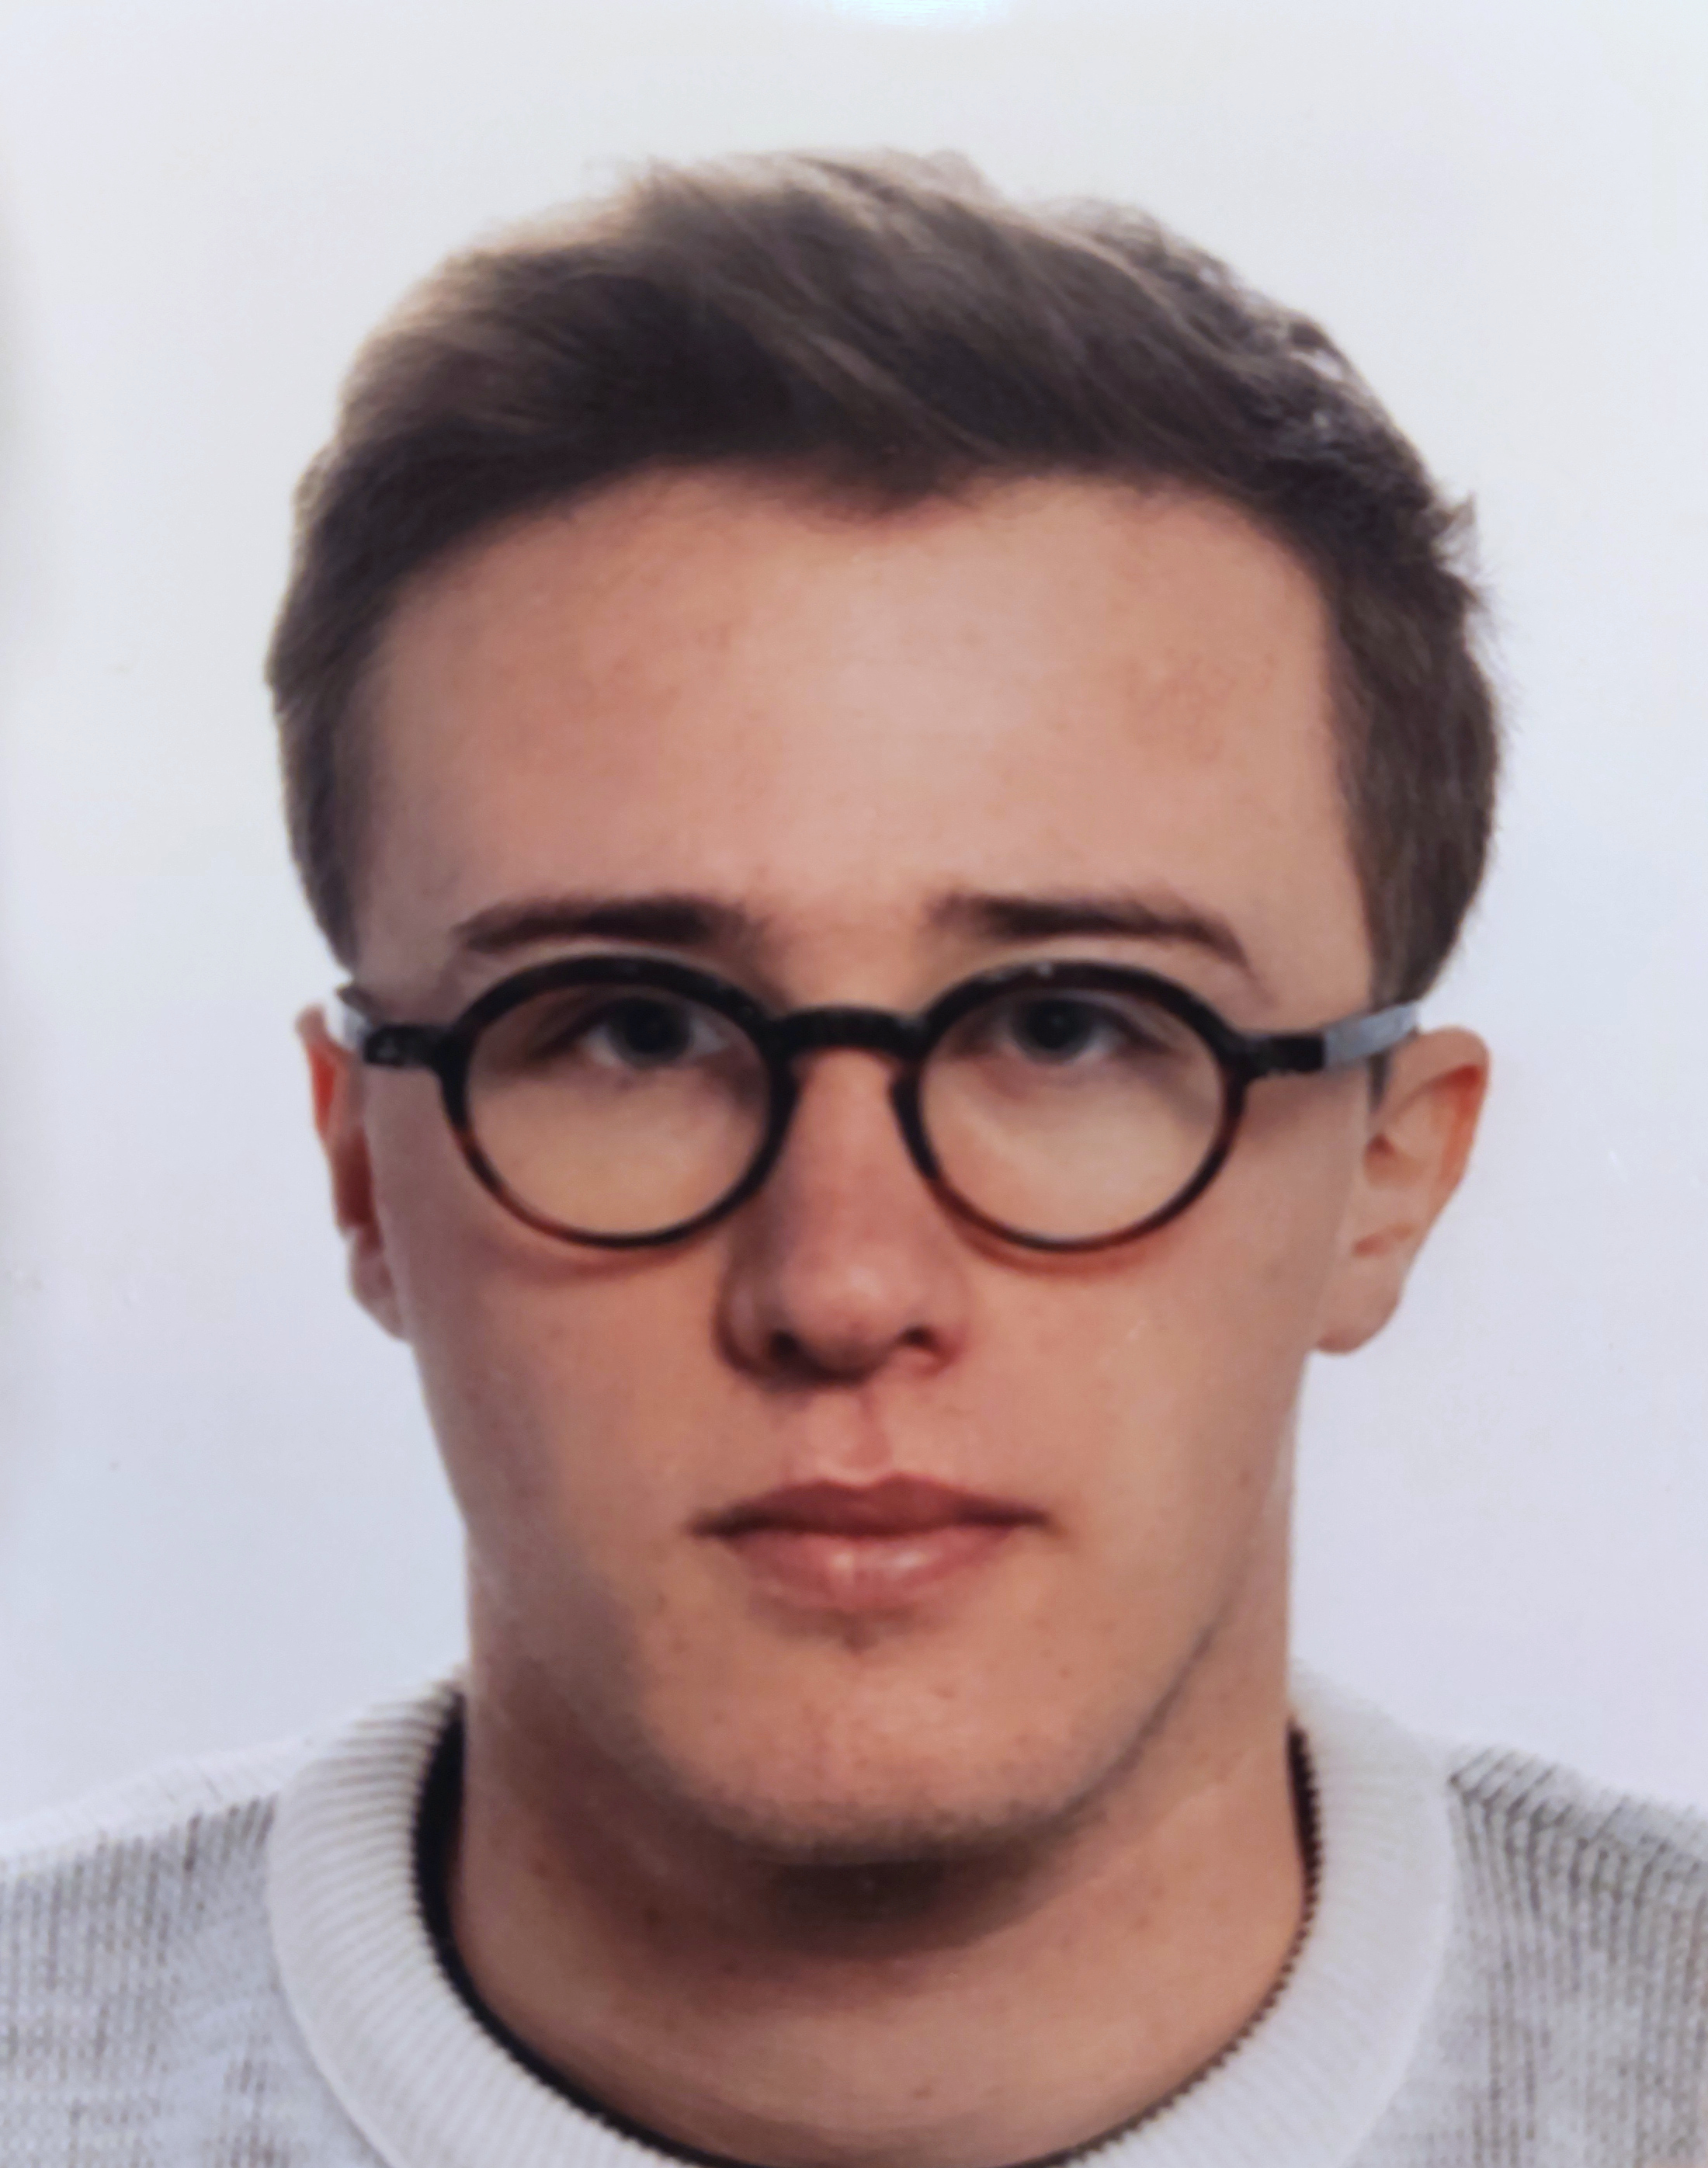
\includegraphics[width=1\columnwidth]{photo.jpg}\\[\baselineskip] % Your photo

Arne Van Den Kerchove \\ % Your name
\Sep
\footnotesize
\url{arne@vandenkerchove.com} \\ % Your email address
\url{arne.vandenkerchove.com} \\ % Your URL
+32 473 32 78 71 \\ % Your phone number
\Sep % Some whitespace
Dijkstraat 33 \\ % Address 1
2480 Dessel \\ % Address 2
Belgium \\ % Address 3
\vfill % Whitespace under this block to push it up under the photo
\end{flushright}
}

%----------------------------------------------------------------------------------------

\begin{document}

\userinformation % Print your information in the left column

\framebreak % End of the first column

%----------------------------------------------------------------------------------------
%	HEADING
%----------------------------------------------------------------------------------------

\cvheading{Arne Van Den Kerchove} % Large heading - your name

\cvsubheading{Computer Science Student} % Subheading - your occupation/specialization

%----------------------------------------------------------------------------------------
%	ABOUT ME
%----------------------------------------------------------------------------------------

\aboutme{About Me}{I am a motivated Computer Science Student at KU Leuven University with interests in open source software and Artificial Intelligence. I volunteer in multiple non-profit organisations, both in Leuven and in my home town. My field of interest is large and I love to discover new experiences and places.}

%----------------------------------------------------------------------------------------
%	EDUCATION 
%----------------------------------------------------------------------------------------

\CVSection{Education}

%------------------------------------------------

\CVItem{2017 - present, KU Leuven University}{Master's Degree in Engineering Sciences: Computer Science - Option Artificial Intelligence (Ongoing)}

\CVItem{2014 - present, KU Leuven University}{Bachelor's Degree in Informatics (Ongoing)}

%\CVItem{2008 - 2014, Sancta Maria Institute Kasterlee}{Modern Languages - Mathematics, option Science}

%------------------------------------------------


\Sep % Extra whitespace after the end of a major section

%----------------------------------------------------------------------------------------
%	EXPERIENCE
%----------------------------------------------------------------------------------------

\CVSection{Professional Experience}

\CVItem{2016 - present, \textit{Freelance Webdeveloper}}{
Currently, I am a self-employed webdeveloper and webdesigner. I use the Drupal CMS and Django Framework to provide personalized websites to my clients.
}

\CVItem{May 2015, \textit{Database Refactoring}, Brabantse Apothekers Federatie}{I was employed to refactor the companies database to a new structure.}

\CVItem{June 2014 - August 2014, \textit{Front-end Webdeveloper}, GBits Webdevelopement}{I was employed to design CSS/HTML templates for the DotNetNuke CMS.}


\Sep % Extra whitespace after the end of a major section

%----------------------------------------------------------------------------------------
%	EXPERIENCE
%----------------------------------------------------------------------------------------

\CVSection{Personal Experience}

\CVItem{February 2016 - present, \textit{Webmaster}, Scientica Leuven vzw}{I manage the computer systems, software and website of the overarching student association Scientica. I am in control of a multi-server system, primarily used for our member database and student course sale system.}

\CVItem{2015 - present, \textit{Responsible Person Webteam}, Wina Leuven vzw}{I lead the technical support team of our student association Wina. I am in charge of a team consisting of 12 volunteers.}

\CVItem{2014 - 2018, \textit{Vice Responsible Person}, Youth Red Cross Retie-Dessel}{
I am a youth leader in our local youth movement. We are an openly accessible youth movement organise by the Belgian Red Cross, that combines playing with first aid education.
}

\CVItem{July 2016, \textit{Sailing Trainee}, The Tall Ships Races}{I participated in the 2016 Tall Ships Races. This is an international and multicultural sailing regatta. I worked and lived  together with people from different countries while sailing from Antwerp to Lisboa.}


\Sep
%----------------------------------------------------------------------------------------
%	COMMUNICATION SKILLS
%----------------------------------------------------------------------------------------

\CVSection{Communication Skills}

{\begin{tabular}{p{1\textwidth}}
		\bluebullet \textit{Native Language}: Dutch \\
		\bluebullet \textit{Full Professional Proficiency}: English, German \\
		\bluebullet \textit{Minimum Professional Proficiency}: French \\
		\bluebullet \textit{Elementary Proficiency}: Spanish, Italian \\
\end{tabular}}

\Sep % Extra whitespace after the end of a major section

%----------------------------------------------------------------------------------------
%	NEW PAGE DELIMITER
%	Place this block wherever you would like the content of your CV to go onto the next page
%----------------------------------------------------------------------------------------

\clearpage % Start a new page

\userinformation % Print your information in the left column

\framebreak % End of the first column

%----------------------------------------------------------------------------------------
%	SKILLS
%----------------------------------------------------------------------------------------

\CVSection{Software Development Skills}

%------------------------------------------------

\CVItem{Programming}
{\begin{tabular}{p{0.15\textwidth} p{0.15\textwidth} p{0.15\textwidth} p{0.15\textwidth}}
\bluebullet Java &  \bluebullet C, C++ & \bluebullet Python & \bluebullet Haskell\\
\bluebullet PHP &  \bluebullet C\# & \bluebullet Matlab & \bluebullet Prolog \\
\bluebullet JQuery 
\end{tabular}}

%------------------------------------------------

\CVItem{Computer Software}
{\begin{tabular}{p{0.15\textwidth} p{0.15\textwidth} p{0.15\textwidth} p{0.15\textwidth}}
 \bluebullet MySQL &  \bluebullet HTML,CSS & \bluebullet \footnotesize Visual Paradigm & \bluebullet Git,Gitlab CI\\
 \bluebullet LaTeX &  \bluebullet Adobe CS6 & \bluebullet R & \bluebullet Server stack\\
\end{tabular}}

%------------------------------------------------

\Sep % Extra whitespace after the end of a major section



\CVSection{Other Qualifications}


\CVItem{\textit{Animator in Youth Work}, Government of Flanders}{}
\CVItem{\textit{First Aid Emergency Worker}, Belgian Red Cross}{}

%----------------------------------------------------------------------------------------
%	INTERESTS
%----------------------------------------------------------------------------------------

\CVSection{Interests}

%------------------------------------------------

\CVItem{Professional}{Artificial intelligence, open source software and opens source software development, webdesign and webdevelopment, declarative programming languages, science and engineering.}

%------------------------------------------------

\CVItem{Personal}{Travelling, first aid and Red Cross, books, guitar, biology.}

%------------------------------------------------

\Sep % Extra whitespace after the end of a major section

%----------------------------------------------------------------------------------------

\end{document}
